\section{ANÁLISIS DE UNA OBRA DODECAFÓNICA: OP. 25}\label{ch:suite}
	\subsection{Series de la Suite op. 25}
		Lo primero que hará un compositor dodecafónico antes de empezar a componer será escoger su serie original. Su elección nunca es una simple cuestión de azar; al contrario, ya que las singularidades de la serie darán un carácter especial a toda la obra. Por ejemplo, el compositor puede escoger una serie con simetrías, y así tendrá series repetidas entre su espectro serial. También puede tener simetrías internas solo en un fragmento de tres o cuatro notas, y de este modo podrá el compositor oscilar entre varias series del espectro que se parezcan entre sí.
		
		({Para un estudio más completo de las relaciones de similitud entre series se recomienda \emph{On the Similarity of Twelve-Tone Rows}, de Tuukka Ilomäki \cite{ilomaki}.})
		
		En la Suite para Piano Op. 25, Schoenberg escoge su serie $\sigma$ para resaltar el intervalo de tritono (6 semitonos). A continuación se observan en negrita los intervalos entre las notas de esta serie, en unidad de semitono:
		
		{$\left(\begin{array}{*{24}c}
			0&&1&&2&&3&&4&&5&&6&&7&&8&&9&&10&&11&\\
			4&\mathbf{1}&5&\mathbf{2}&7&\mathbf{6}&1&\mathbf{5}&6&\mathbf{9}&3&\mathbf{5}&8&\mathbf{6}&2&\mathbf{9}&11&\mathbf{1}&0&\mathbf{9}&9&\mathbf{1}&10&\mathbf{6}\end{array}\right)$}
				
		Presenta repeticiones triples de los intervalos de tritono (6), de sexta mayor (9) y de segunda menor o semitono (1): los intervalos más disonantes; una repetición doble de cuarta justa (5), y un intervalo de segunda mayor (2); además de una consecución de intervalos repetida: 9 -- 1 -- 9 -- 1. Como se forma el intervalo de tritono al enlazar la serie original con una serie que empiece por la misma nota, se tiene en cuenta el intervalo de tritono (6) al final. En el dodecafonismo se evitan deliberadamente los intervalos de tercera mayor (4), ya que estos son la base de la eludida armonía tonal. \label{serie25}
		
		El intervalo de tritono tiene la particularidad de no modificarse en la inversión y transportación k = 6, por lo que estos intervalos aparecen en los lugares originales, mientras que en los procedimientos de retrogradación y retrogradación inversa ocupan sus lugares en retrógrado. En particular, Schoenberg utiliza entre los seis movimientos de la Suite solamente las ocho series de todo el espectro serial que cumplen estos requisitos: T$^0$, T$^6$, I, IT$^6$, R, RT$^6$, RI y RIT$^6$, que podemos observar %en el Anexo \ref{app:series}, página \pageref{app:series}.
		a continuación:
		
		\chapter{Series de la Suite Op. 25}
	\label{app:series}
	
	\newpage
	$$\text{T}^0=\left(\begin{matrix}0&1&2&3&4&5&6&7&8&9&10&11\\4&5&7&1&6&3&8&2&11&0&9&10\\\end{matrix}\right)$$
	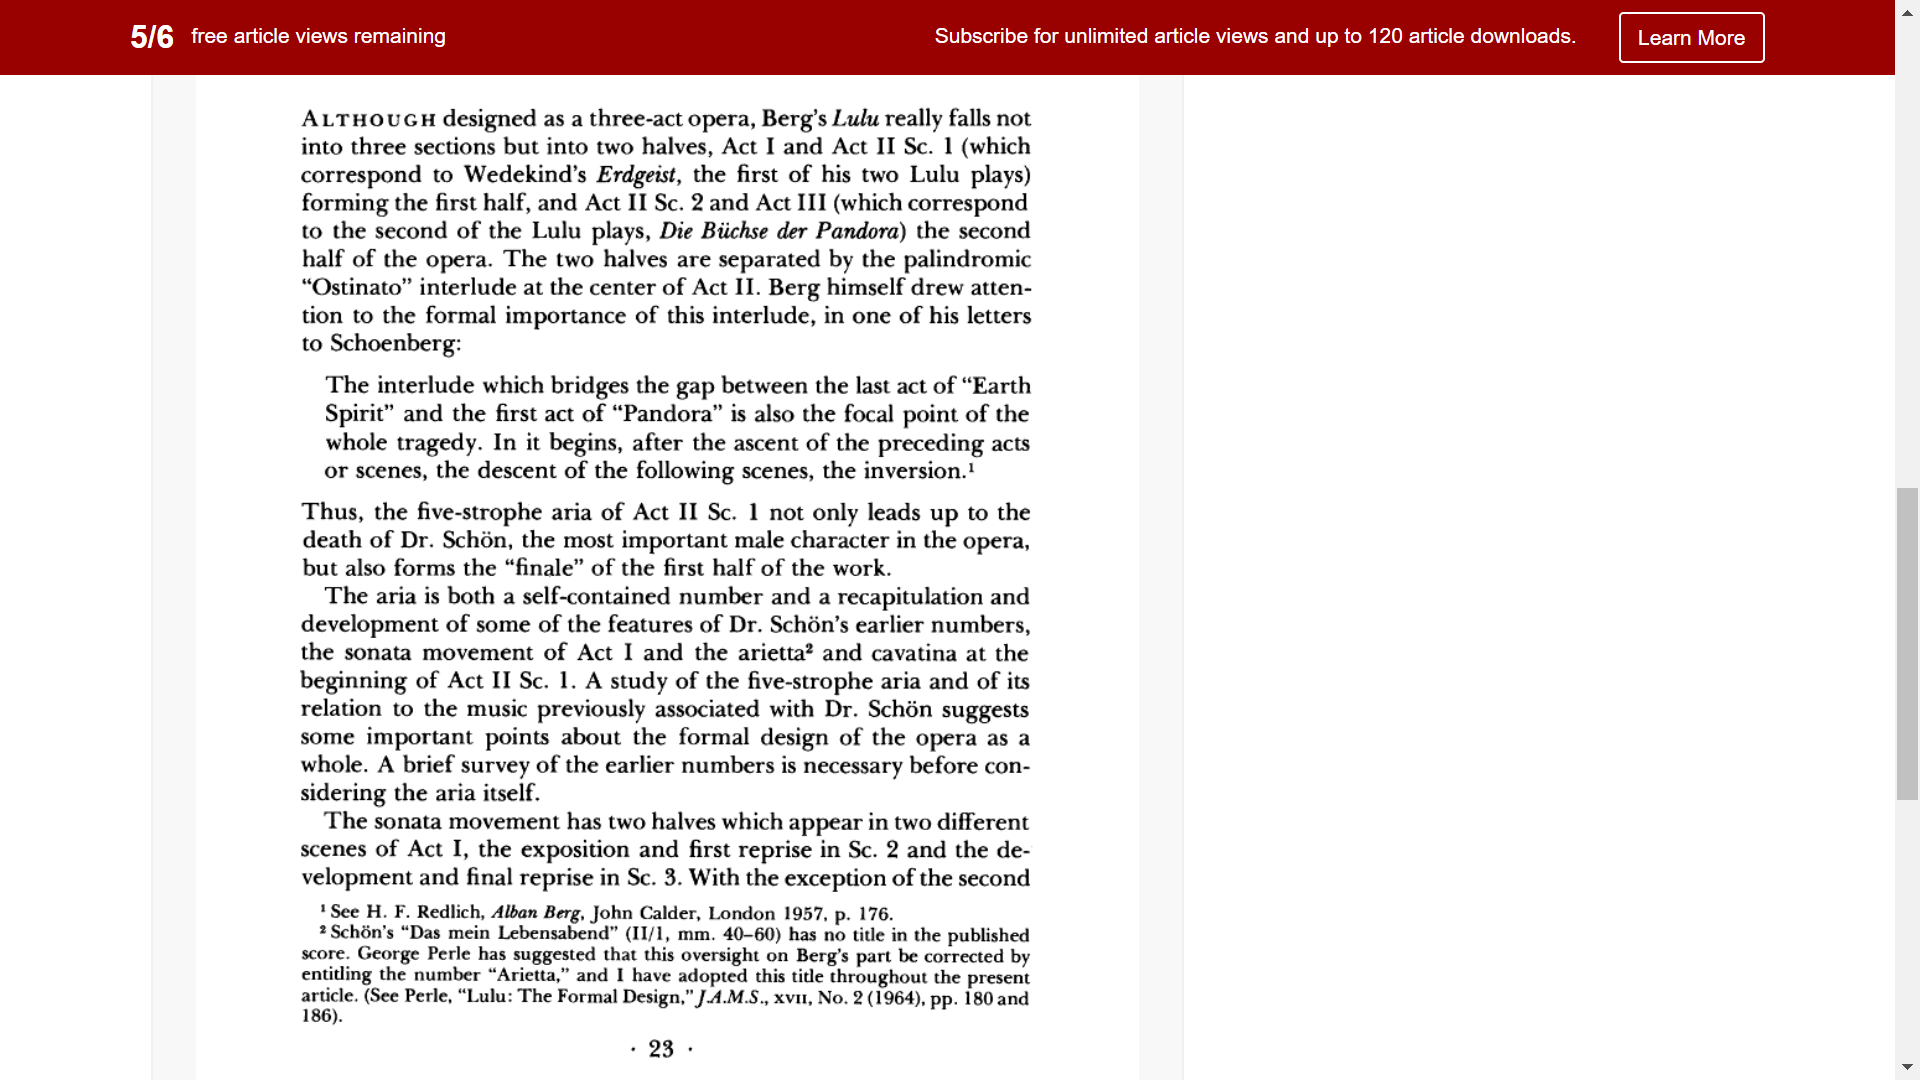
\includegraphics[width=\textwidth]{1.png}
	\bigskip\bigskip
	$$\text{T}^6=\left(\begin{matrix}0&1&2&3&4&5&6&7&8&9&10&11\\10&11&1&7&0&9&2&8&5&6&3&4\\\end{matrix}\right)$$
	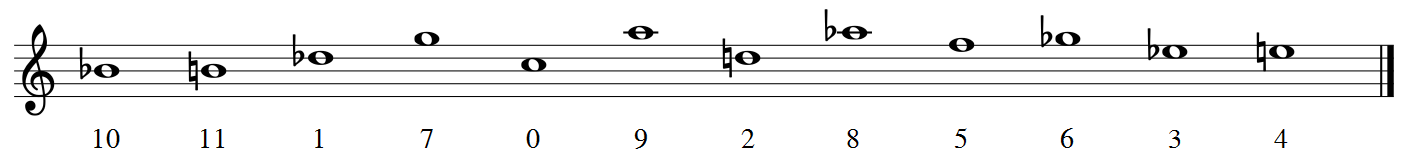
\includegraphics[width=\textwidth]{2.png}
	\bigskip\bigskip
	$$\text{IT}^0=\left(\begin{matrix}0&1&2&3&4&5&6&7&8&9&10&11\\4&3&1&7&2&5&0&6&9&8&11&10\\\end{matrix}\right)$$
	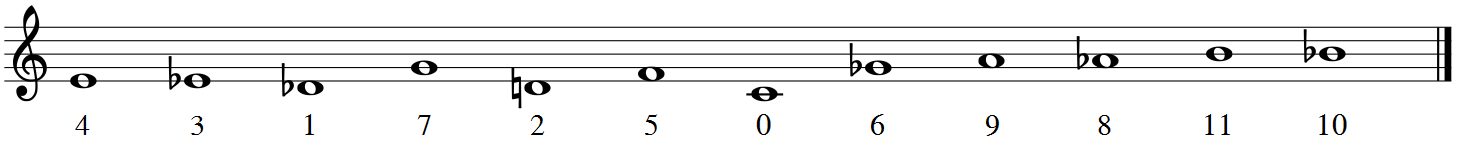
\includegraphics[width=\textwidth]{4.png}
	\bigskip\bigskip
	$$\text{IT}^6=\left(\begin{matrix}0&1&2&3&4&5&6&7&8&9&10&11\\10&9&7&1&8&11&6&0&3&2&5&4\\\end{matrix}\right)$$
	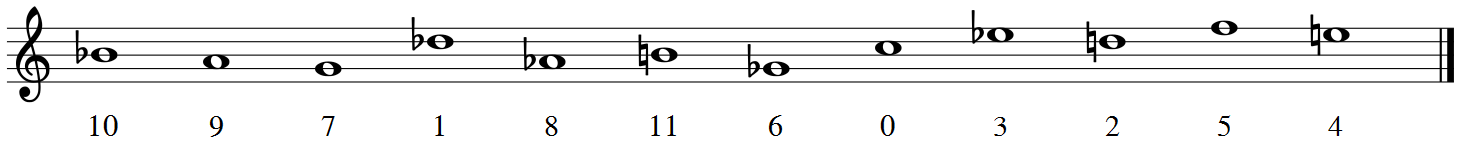
\includegraphics[width=\textwidth]{6.png}
	\newpage
	$$\text{RT}^0=\left(\begin{matrix}0&1&2&3&4&5&6&7&8&9&10&11\\10&9&0&11&2&8&3&6&1&7&5&4\\\end{matrix}\right)$$
	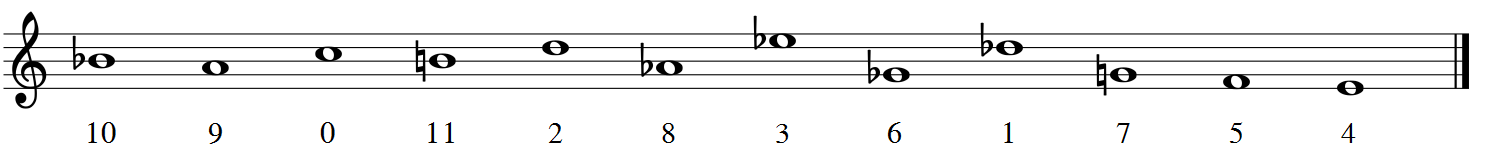
\includegraphics[width=\textwidth]{3.png}
	\bigskip\bigskip
	$$\text{RT}^6=\left(\begin{matrix}0&1&2&3&4&5&6&7&8&9&10&11\\4&3&6&5&8&2&9&0&7&1&11&10\\\end{matrix}\right)$$
	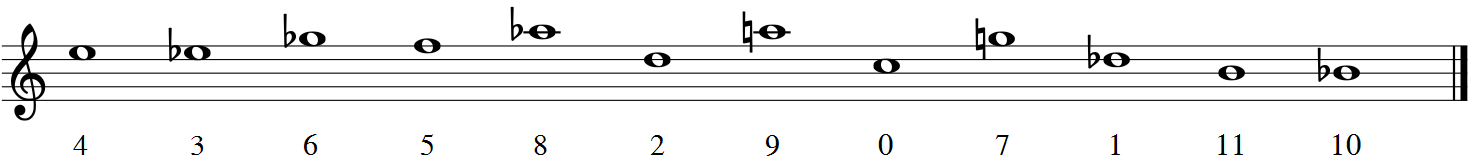
\includegraphics[width=\textwidth]{7.png}
	\bigskip\bigskip
	$$\text{IRT}^0=\left(\begin{matrix}0&1&2&3&4&5&6&7&8&9&10&11\\10&11&8&9&6&0&5&2&7&1&3&4\\\end{matrix}\right)$$
	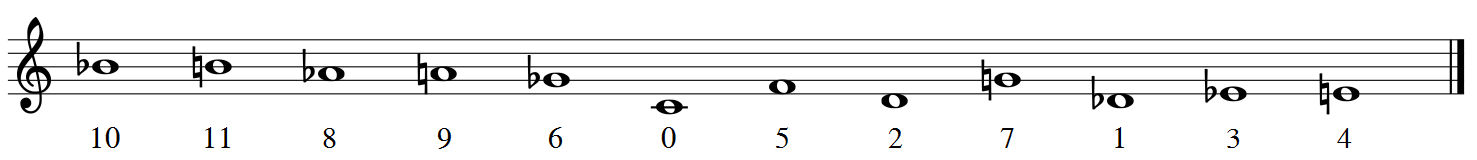
\includegraphics[width=\textwidth]{5.png}
	\bigskip\bigskip
	$$\text{IRT}^6=\left(\begin{matrix}0&1&2&3&4&5&6&7&8&9&10&11\\4&5&2&3&0&6&11&8&1&7&9&10\\\end{matrix}\right)$$
	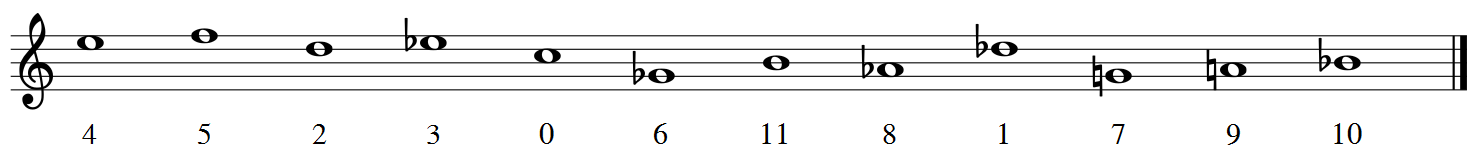
\includegraphics[width=\textwidth]{8.png}
		
		Estas series tienen muchos elementos en común: todas comienzan o acaban por Mi$\natural$ o por Si$\flat$, lo que permite enlazar unas series con otras por medio del unísono o del tritono; se mantienen los intervalos de tritono en sus lugares originales o retrógrados, y coinciden en las dos primeras y las dos últimas notas dos a dos.
		
		Se han realizado estudios -- como el de Martha Hyde \cite{hyde} -- en los que se limitan las series utilizadas en la Suite a cuatro: T$^0$, T$^6$, I e IT$^6$, pero ya que el objetivo de este texto no es analizar la obra entera se dejará esta cuestión para análisis posteriores.
		
	\subsection{Descripción de la Suite op. 25}
		Schoenberg realiza en la serie $\sigma$ una partición triple; es decir, la serie se divide en tres tetracordios, y cada uno de ellos contiene un intervalo de tritono. El último tetracordio, si se retrograda, consta de las notas 10 -- 9 -- 0 -- 11, que en notación germánica es la secuencia BACH. Esto puede ser un homenaje al compositor Johann Sebastian Bach (1685--1750), ya que Schoenberg admiraba a los grandes compositores anteriores a él por las estructuras formales de sus obras.
		%
		\cite{xiao}
		
		Otro posible homenaje a Bach y sus contemporáneos barrocos es precisamente la forma de la obra: es una Suite, género cultivado durante los siglos XVII y XVIII que se compone de una variedad de danzas. La Suite de Schoenberg está formada por seis danzas: un Preludio, una Gavota, una Musette, un Intermezzo -- que no tiene influencia barroca sino más bien de Brahms, otro modelo para Schoenberg --, un Minueto con Trío y una Giga. Además, el estilo, la textura -- contrapuntística, típicamente barroca -- y la estructura de cada danza se corresponden con los estilos, texturas y estructuras de las danzas homónimas del periodo bachiano.
        
        Por ser ésta su primera obra totalmente dodecafónica, Schoenberg la utilizó como una muestra al mundo de las posibilidades de su nuevo método compositivo. Fue también por lo que tomó un formato tan variado como una Suite: así podía en una misma obra componer con estilos tan distintos como los de las distintas danzas.
        
        Al componer la obra, Schoenberg trata cada tetracordio como una subunidad individual. Los superpone contra otras series del espectro también divididas, o utiliza sus notas como un solo acorde cuatríada. Estas divisiones no sólo sirven para hacer la serie más reconocible o añadir cohesión a la obra, sino que además facilitan el desarrollo de la serie específicamente en el estilo de cada danza.
		
	\subsection{Análisis de la Musette}
	\label{musette}
		En el tercer movimiento de la Suite, la Musette, Schoenberg recrea la danza barroca que toma su nombre del instrumento homónimo: la \emph{cornamusa}, de la familia de la gaita. La música compuesta para estos instrumentos suele consistir en una melodía acompañada por una nota pedal, que se traduce aquí en la presencia de un bordón sobre el Sol$\natural$ (nota 7). Esta nota se extrae de cada una de las series utilizadas y se forma con ella un ostinato rítmico en la mano izquierda del piano. Con el resto de sonidos de cada serie, Schoenberg vuelve a emular el estilo de la danza barroca y articula un discurso polifónico a dos voces con ritmos esencialmente cortos.
		
		A partir de la doble barra del compás 9, el Re$\flat$ (nota 1) acompaña a Sol$\natural$ y ambos crean un doble bordón en la mano izquierda. La elección de esas dos notas está estrechamente relacionada con la tradicional relación de quinta justa formada por Sol$\natural$ y Re$\natural$ en la música tonal. Schoenberg sustituye las quintas justas tonales por los tritonos dodecafónicos, subrayando aún más su <<emancipación de la disonancia>>.
		
		Además de las similitudes texturales, rítmicas y armónicas, la Musette de Schoenberg comparte estructura formal con las danzas barrocas. Y esta semejanza es quizás la más notable, ya que fue la búsqueda de estructura formal lo que inspiró a Schoenberg a desarrollar su método compositivo. La Musette barroca, como todos los movimientos de danza, presenta una estructura binaria con simetría tonal: empieza y acaba por la misma tonalidad, mientras que el centro es zona de desarrollo. Schoenberg despoja de funcionalidad tonal a esa simetría, madre de la forma sonata, y la aplica a su composición dodecafónica.
		
		En este movimiento se pueden diferenciar a simple vista tres secciones, divididas en los compases 9 y 20, debido a cambios de textura, figuración y tempo. En la segunda sección se le añade melodía a la mano izquierda del piano, dejando más camuflado el bordón que en la primera sección, además de que éste se vuelve doble, mientras que vuelve a aparecer claramente en la tercera sección. También en la segunda sección aparece una nueva figuración, que es la semicorchea; y, por último, en los dos compases de división aparecen dos \emph{a tempo}, que marcan el final de las dos primeras secciones tras dos zonas de variabilidad rítmica.
		%
		\cite{clercq}
		
		Para que esta estructura tríptica sea una forma binaria, la primera y la última parte deben mantener un parecido, que se observa a través del análisis de las series utilizadas en el movimiento. Estas series son T$^0$, T$^6$, I e IT$^6$.
		
		En la Musette, Schoenberg hace un uso casi absoluto de la tripartición serial, hasta el punto de individualizar los tetracordios por separado y concederles privilegios seriales, como la retrogradación. Por ejemplo, en el compás 7, en la voz inferior de la mano derecha aparece el tetracordio 4 -- 5 -- 2 -- 3, que es o bien el primer tetracordio de RIT$^6$ o la retrogradación del tercer tetracordio de IT$^6$, mientras que los otros dos tetracordios de IT$^6$, 10 -- 9 -- 7\footnote{La nota 7 aparece como bordón y no en la misma voz que el resto del tetracordio, por lo que su posición es también excepcional.} -- 1 en la voz superior y 8 -- 11 -- 6 -- 0 en la mano izquierda, aparecen en el orden correcto. Entonces no se puede analizar el compás como RIT$^6$, sino indicar que hay una alteración puntual de IT$^6$.
		
		Por tanto, es muy complicado analizar esta obra en su totalidad, ya que la flexibilidad en la ordenación de los tetracordios puede generar situaciones muy ambiguas. Debido a estas fragmentaciones y a las variadas combinaciones de tetracordios originales y retrógrados, se escucha un área de desarrollo hacia la sección media del movimiento. En cambio, las series al principio y al final de la pieza se presentan casi íntegramente, como una exposición y reexposición. He aquí un vínculo con la simetría de las formas binarias tonales.
		%
		\cite{clercq}
		
		Es más, incluso el orden de las series utilizadas en la primera y en la última sección coinciden, exceptuando dos repeticiones consecutivas y las series T$^0$ finales, que actúan como una cadencia serial:
		
		\[\begin{array}{*{12}c}
			\mathbf{c}.\mathbf{1}&\text{T}^0&\text{IT}^6&\text{T}^6&\text{I}&\text{T}^0&\text{I}&\text{T}^6&
				\begin{matrix}\text{IT}^6&\text{IT}^6\\
				\end{matrix}
			&&&\mathbf{c}.\mathbf{9}\\
			\mathbf{c}.\mathbf{22}&\text{T}^0&\text{IT}^6&\text{T}^6&\text{I}&\text{T}^0&
				\begin{matrix}
				\text{I}&\text{I}\\
				\end{matrix}
			&\text{T}^6&\text{IT}^6&\text{T}^0&\text{T}^0&\mathbf{c}.\mathbf{31}\\\end{array}\]
		
		A continuación se encuentra el análisis serial completo de la Musette:
		
		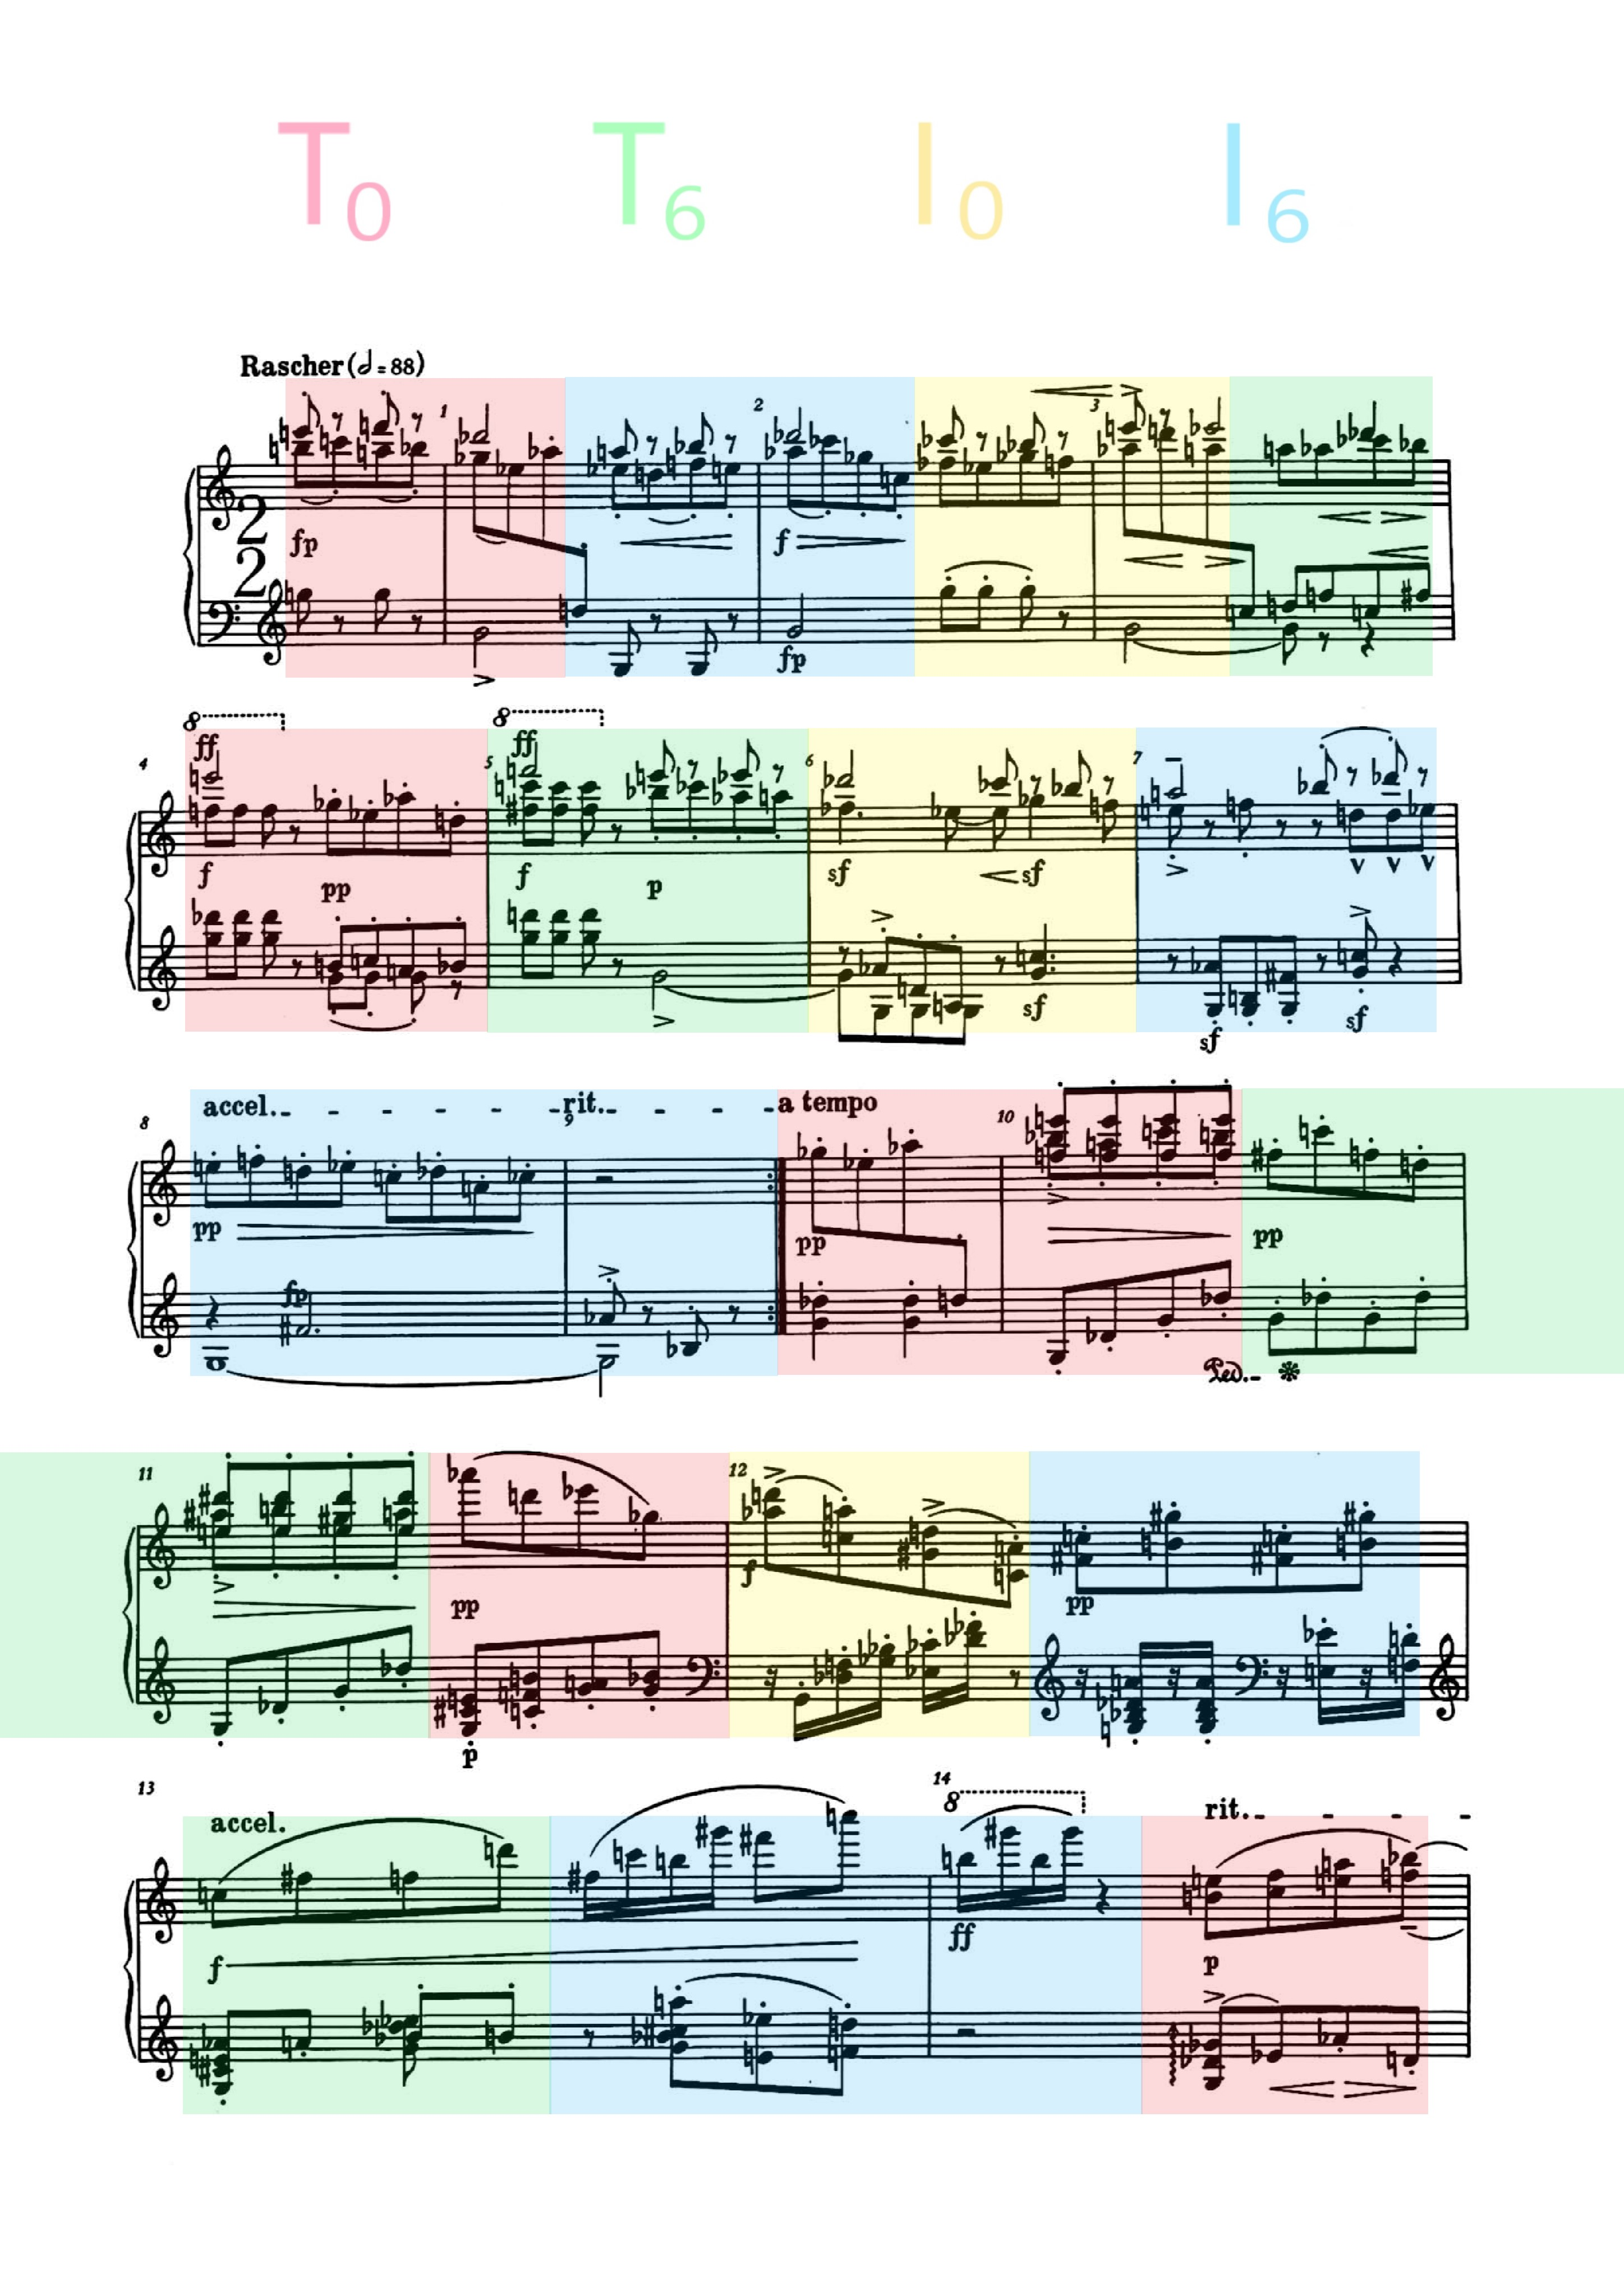
\includegraphics[width=15cm]{9.jpg}
		
		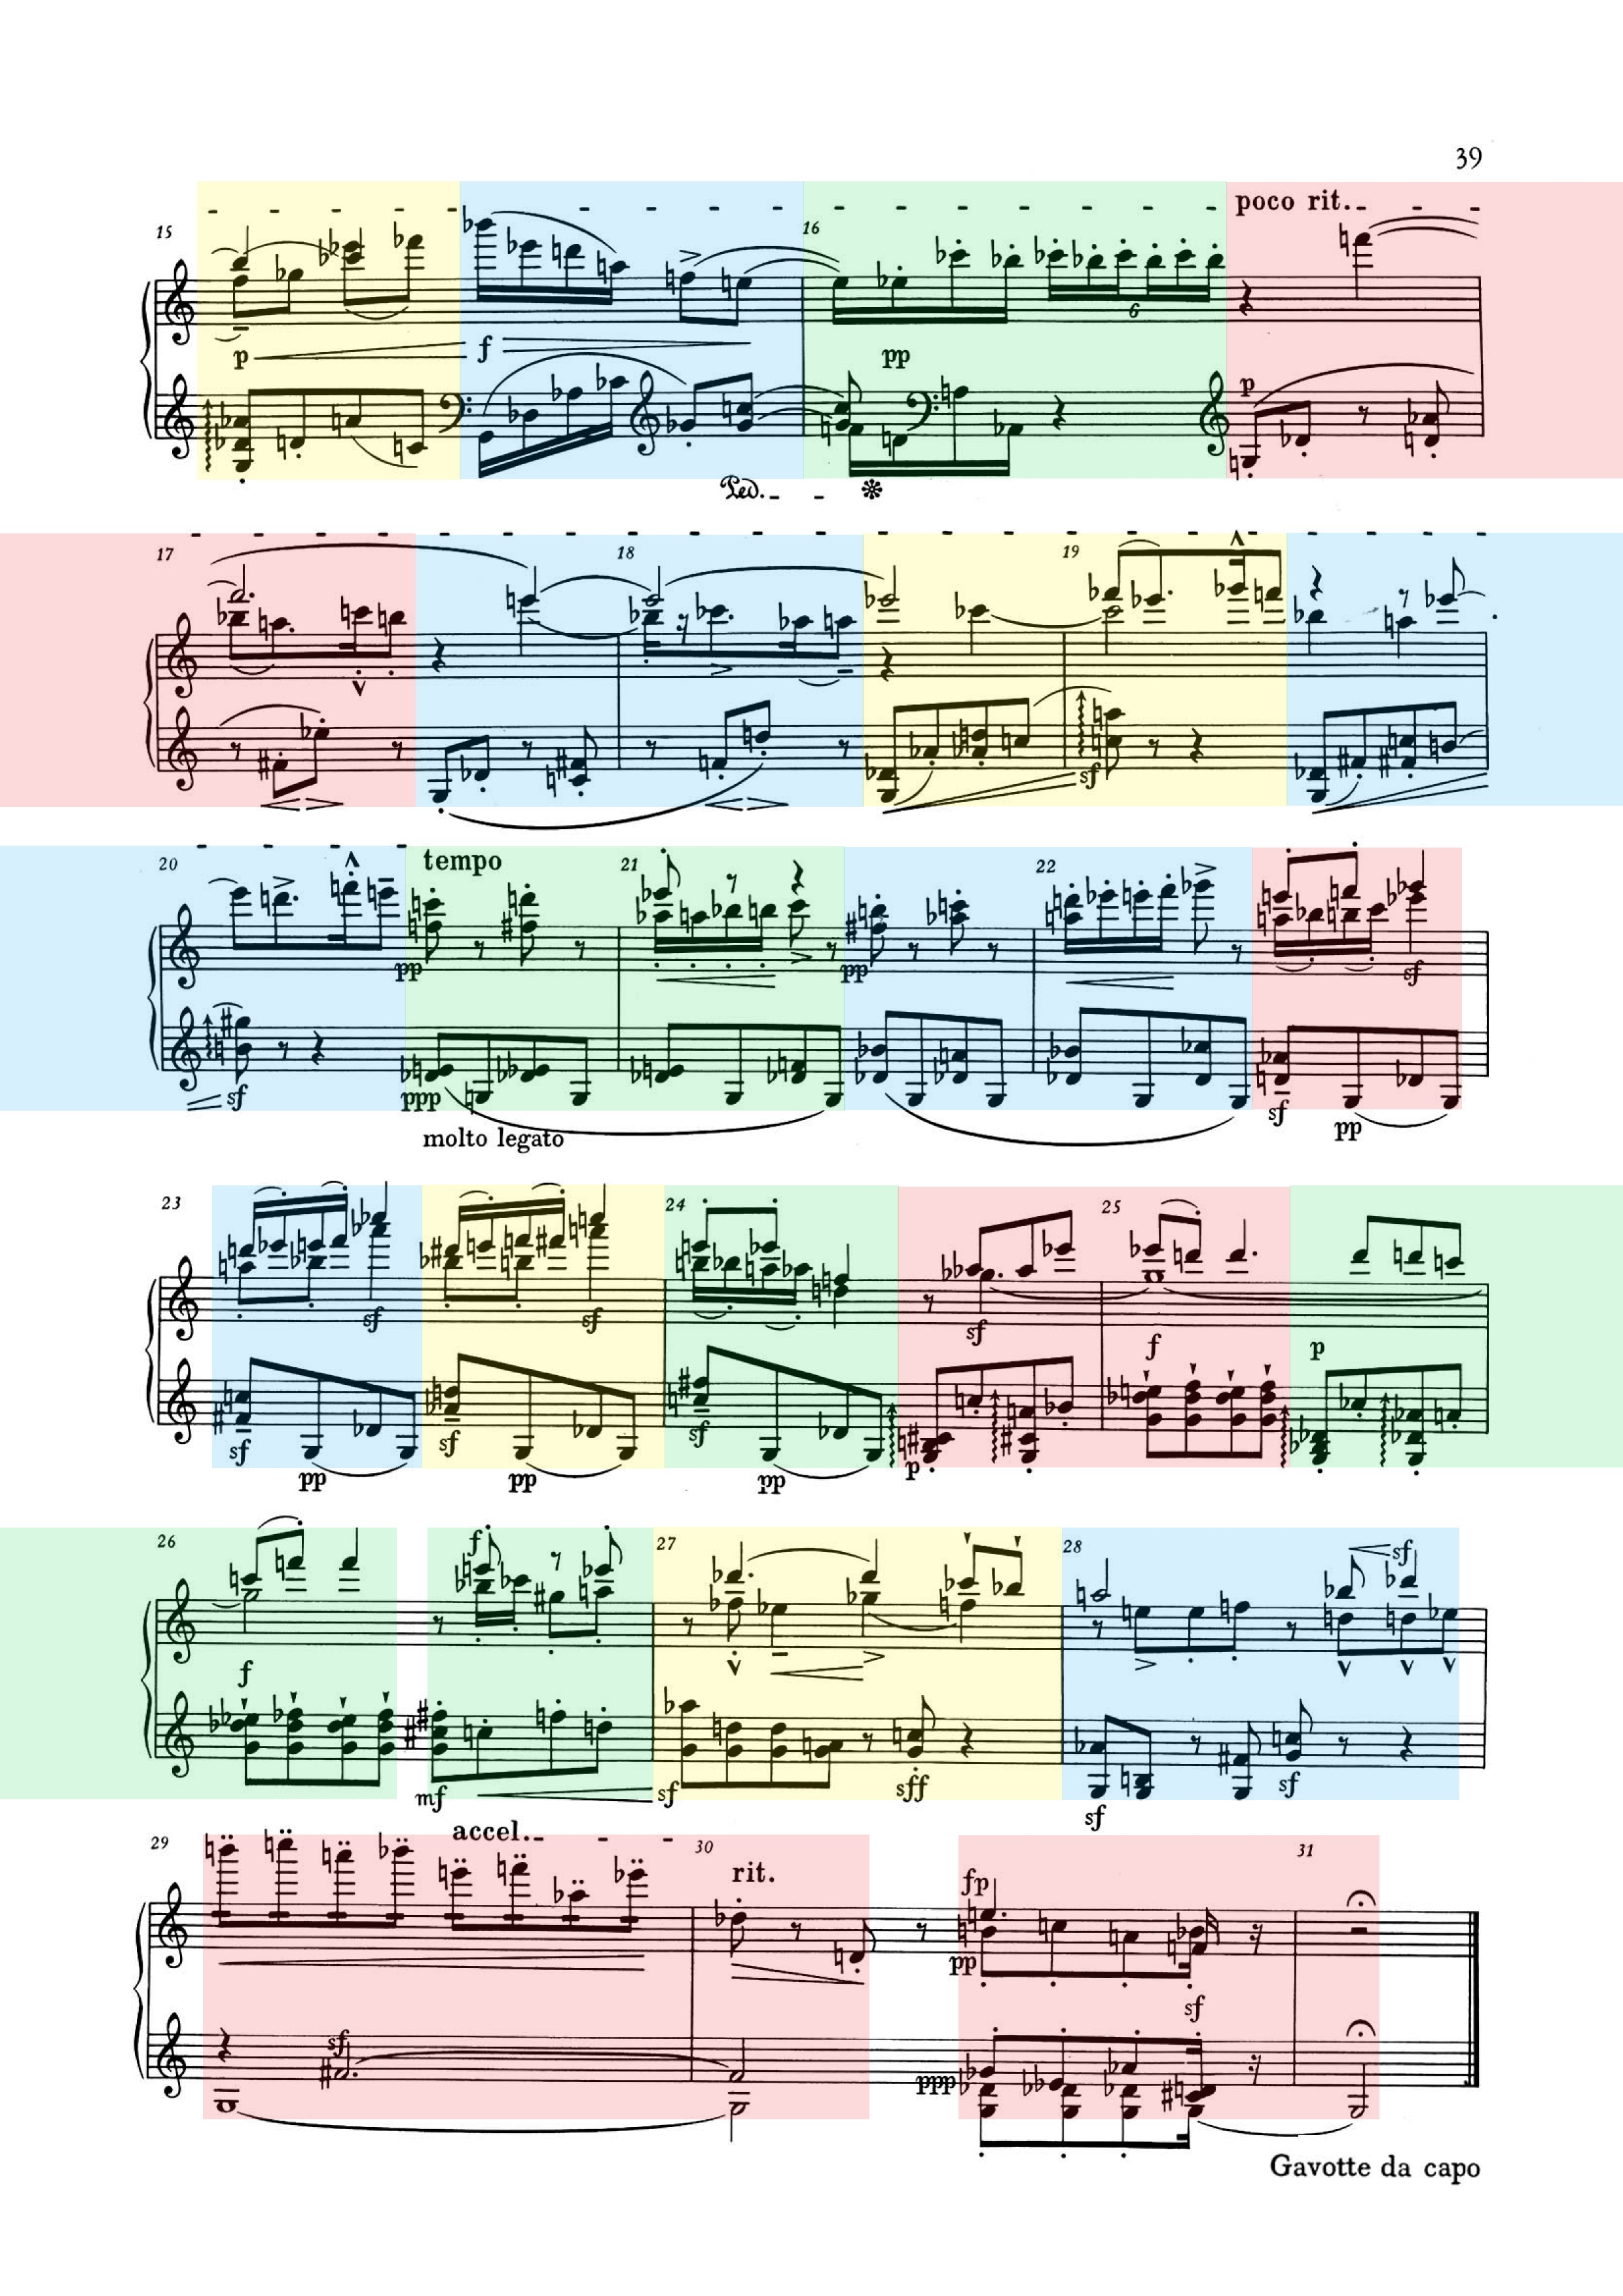
\includegraphics[width=15cm]{10.jpg}